% Search for all the places that say "PUT SOMETHING HERE".

\documentclass[11pt]{article}
\usepackage{amsmath,textcomp,amssymb,graphicx,enumerate,hyperref,enumitem,mathtools,tikz-qtree,listings}

\def\Name{Jonathan Sun}  % Your name
\def\SID{25020651}  % Your student ID number
\def\Homework{1} % Number of Homework
\def\Session{Fall 2017}


\title{CS170 --- \Session --- Homework \Homework \space Solutions}
\author{\Name, SID \SID}
\markboth{CS170 --- \Session --- Homework \Homework \space --- \Name}{CS170 --- \Session --- Homework \Homework --- \Name}
\pagestyle{myheadings}
\date{}

\def\endproofmark{$\Box$}
\newenvironment{proof}{\par{\bf Proof:}}{\endproofmark\smallskip}
\newenvironment{FourPartSolution}{\par{\bf Four-Part Solution:}}{\smallskip}
\newenvironment{mainIdea}{\par{\bf Main Idea:}}{\smallskip}
\newenvironment{pseudocode}{\par{\bf Pseudocode:}}{\smallskip}
\newenvironment{proofOfCorrectness}{\par{\bf Proof of Correctness:}}{\endproofmark\smallskip}
\newenvironment{runTime}{\par{\bf Run Time:}}{\smallskip}
\newenvironment{justification}{\par{\bf Justification:}}{\smallskip}

\usepackage[margin=1in]{geometry}



\begin{document}
\maketitle

Collaborators: Kevin Vo, Aleem Zaki, Jeremy Ou

\section*{1. Course Syllabus}
\begin{enumerate}[label=(\alph*)]
\item
Not OK. Cheating includes: `Receiving help on homeworks from students who have taken the course in previous semesters.' I got this quote from the syllabus at `\url{https://berkeley-cs170.github.io/fa17-www/policies.html}'.

\item
Not OK. Cheating includes: `Sharing your solutions, or partial solutions, with another student, even with the explicit understanding that they won't be copied or with students in your homework group.' I got this quote from the syllabus at `\url{https://berkeley-cs170.github.io/fa17-www/policies.html}'.

\item
Not OK. Cheating includes: `Searching the Internet for a solution to the exact problem we gave you on a homework.' The fact that you cited the source does not mean that you have not cheated. I got the quote from the syllabus at `\url{https://berkeley-cs170.github.io/fa17-www/policies.html}'.

\item
OK. Cheating includes: `Searching the Internet for a solution to the exact problem we gave you on a homework' and `Using ideas from any external source without citing it.' However, since you have not searched the Internet for a solution to the exact problem but was looking up Dijkstra's Algorithm, you have not broken the rule for the first part. You have also cited the source so you have not broken the rule for the second part. I got the quotes from the syllabus at `\url{https://berkeley-cs170.github.io/fa17-www/policies.html}'.

\item
OK. Cheating includes: `Telling someone who is not in your homework group how to solve a homework problem', `Using ideas from any external source without citing it', and `Sharing your solutions, or partial solutions, with another student, even with the explicit understanding that they won't be copied or with students in your homework group.' However, since you have been actively involved in the conversation between the student and the TA, this does not break the third part of the rule because the TA and the student are not sharing solutions or partial solutions. Furthermore, if you write down the other student as a collaborator, then you will not be breaking the first part of the rule since the other student is in your homework group. Last, if you cite the TA and the other student, you won't be breaking the second part of the rule. I got the quotes from the syllabus at `\url{https://berkeley-cs170.github.io/fa17-www/policies.html}'.

\end{enumerate}



\newpage
\section*{2. Asymptotic Complexity Comparisons}
\begin{enumerate}[label=(\alph*)]
\item
(iii) $f_3(n) = 12$ \\
(vii) $f_7(n) = \log_2n$ \\
(ii) $f_2(n) = n^{\frac{1}{3}}$ \\
(v) $f_5(n) = \sqrt{n}$ \\
(iv) $f_4(n) = 2^{\log_2n}$ \\
(ix) $f_9(n) = n^3$ \\
(viii) $f_8(n) = 2^{\sqrt{n}}$ \\
(vi) $f_6(n) = 2^n$ \\
(i) $f_1(n) = 3^n$

\item
\begin{enumerate}[label=(\roman*)]
\item
$f = \Theta(g)$.
\begin{proof}
This is because $\displaystyle{\lim_{n \to \infty} \frac{f(n)} {g(n)}} = \displaystyle{\lim_{n \to \infty} \frac{\log_3n} {\log_4n}} = \displaystyle{\lim_{n \to \infty} \frac{\frac{1} {n\ln{3}}} {\frac{1} {n\ln{4}}}} = \displaystyle{\lim_{n \to \infty} \frac{n\ln{4}} {n\ln{3}}} = \displaystyle{\lim_{n \to \infty} \frac{\ln{4}} {\ln{3}}} = \frac{\ln{4}} {\ln{3}}$. Since this limit gives me a constant, then $f \in \Theta(g)$.
\end{proof}

\item
$f = O(g)$.
\begin{proof}
This is because $\displaystyle{\lim_{n \to \infty} \frac{f(n)} {g(n)}} = \displaystyle{\lim_{n \to \infty} \frac{n\log{(n^4)}} {n^2\log{(n^3)}}} = \displaystyle{\lim_{n \to \infty} \frac{4n\log{n}} {3n^2\log{n}}} = \displaystyle{\lim_{n \to \infty} \frac{4} {3n}} = 0$. Since this limit gives me 0, then $f$ grows slower than $g$ and so $f \in O(g)$.
\end{proof}

\item
$f = \Omega(g)$.
\begin{proof}
This is because $\displaystyle{\lim_{n \to \infty} \frac{f(n)} {g(n)}} = \displaystyle{\lim_{n \to \infty} \frac{\sqrt{n}} {(\log{n})^3}} = \displaystyle{\lim_{n \to \infty} \frac{\frac{1} {2\sqrt{n}}} {\frac{3(\log{n})^2} {n\ln{2}}}} = \displaystyle{\lim_{n \to \infty} \frac{\sqrt{n}\ln{2}} {6(\log{n})^2}} = \displaystyle{\lim_{n \to \infty} \frac{\ln{2}(\frac{1} {2\sqrt{n}})} {\frac{12\log{n}} {n\ln{2}}}} = \displaystyle{\lim_{n \to \infty} \frac{n(\ln{2})^2} {24\sqrt{n}\log{n}}} = \displaystyle{\lim_{n \to \infty} \frac{(\ln{2})^2\sqrt{n}} {24\log{n}}} = \displaystyle{\lim_{n \to \infty} \frac{\frac{(\ln{2})^2} {2\sqrt{n}}} {\frac{24} {n\ln{2}}}} = \displaystyle{\lim_{n \to \infty} \frac{(\ln{2})^3n} {48\sqrt{n}}} = \displaystyle{\lim_{n \to \infty} \frac{(\ln{2})^3\sqrt{n}} {48}} = \infty$. Since this limit gives me $\infty$, then $f$ grows faster than $g$ and so $f \in \Omega(g)$.
\end{proof}

\item
$f = \Theta(g)$.
\begin{proof}
This is because $\displaystyle{\lim_{n \to \infty} \frac{f(n)} {g(n)}} = \displaystyle{\lim_{n \to \infty} \frac{2^n} {2^{n + 1}}} = \displaystyle{\lim_{n \to \infty} \frac{2^n} {2(2^n)}} = \displaystyle{\lim_{n \to \infty} \frac{1} {2}} = \frac{1} {2}$. Since this limit gives me a constant, then $f \in \Theta(g)$.
\end{proof}

\item
$f = \Omega(g)$.
\begin{proof}
This is because $\displaystyle{\lim_{n \to \infty} \frac{f(n)} {g(n)}} = \displaystyle{\lim_{n \to \infty} \frac{n} {(\log{n})^{\log{\log{n}}}}} = \displaystyle{\lim_{n \to \infty} \frac{1} {(\frac{\ln{(\log{n})}} {(\ln{2})^2n\log{n}} + \frac{\log{\log{n}}} {n\ln{n}})\log{n}^{\log{\log{n}}}}} = \infty$. Since this limit gives me $\infty$, then $f$ grows faster than $g$ and so $f \in \Omega(g)$.
\end{proof}

\item
$f = \Theta(g)$.
\begin{proof}
This is because $\displaystyle{\lim_{n \to \infty} \frac{f(n)} {g(n)}} = \displaystyle{\lim_{n \to \infty} \frac{n + \log{n}} {n + (\log{n})^2}} = \displaystyle{\lim_{n \to \infty} \frac{1 + \frac{1} {n\ln{2}}} {1 + \frac{2\log{n}} {n\ln{2}}}} = \displaystyle{\lim_{n \to \infty} \frac{\frac{n\ln{2} + 1} {n\ln{2}}} {\frac{n\ln{2} + 2\log{n}} {n\ln{2}}}} = \displaystyle{\lim_{n \to \infty} \frac{n\ln{2} + 1} {n\ln{2} + 2\log{n}}} = \displaystyle{\lim_{n \to \infty} \frac{\ln{2}} {\ln{2} + \frac{2} {n\ln{2}}}} = \displaystyle{\lim_{n \to \infty} \frac{\ln{2}} {\frac{n(\ln{2})^2 + 2} {n\ln{2}}}} = \displaystyle{\lim_{n \to \infty} \frac{\ln{2}} {\frac{n(\ln{2})^2 + 2} {n\ln{2}}}} = \displaystyle{\lim_{n \to \infty} \frac{n(\ln{2})^2} {n(\ln{2})^2 + 2}} = \displaystyle{\lim_{n \to \infty} \frac{(\ln{2})^2} {(\ln{2})^2}} = 1$. Since this limit gives me a constant, then $f \in \Theta(g)$.
\end{proof}

\item
$f = O(g)$.
\begin{proof}
This is because $\displaystyle{\lim_{n \to \infty} \frac{f(n)} {g(n)}} = \displaystyle{\lim_{n \to \infty} \frac{\log{(n!)}} {n\log{n}}} = \displaystyle{\lim_{n \to \infty} \frac{\log{(n!)}} {\log{n^n}}} = \displaystyle{\lim_{n \to \infty} \frac{\log{({\prod\limits_{i = 1}^{n} i})}} {\log{({\prod\limits_{i = 1}^{n} n})}}} = \displaystyle{\lim_{n \to \infty} \frac{\log{(1 * 2 * 3 * ... * (n - 2) * (n - 1) * n)}} {\log{(n * n * n * ... * n * n * n)}}} = 0$. This gives $0$ because $n$ will always be greater than $(n - 1)$ so $\log{({\prod\limits_{i = 1}^{n} i})} \leq \log{({\prod\limits_{i = 1}^{n} n})}$ and therefore the numerator will always be smaller than or equal to the denominator. Since this limit gives me 0, then $f$ grows slower than $g$ and so $f \in O(g)$.
\end{proof}

\end{enumerate}

\item
$f_1 = 2^n$ \\
$f_2 = n$ \\
When plugging in $f_1 = 2^n$, $\sum\limits_{i = 1}^{n} f(i) = \sum\limits_{i = 1}^{n} 2^i = 2^1 + 2^2 + 2^3 + ... + 2^n$. Evaluating this will give $2^n$. When plugging in $f_1 = 2^n$, $\Theta(f(n)) = \Theta(2^n)$. Since $2^n = 2^n$, $f_1 = 2^n$ is a function such that the equality holds. \\
When plugging in $f_2 = n$, $\sum\limits_{i = 1}^{n} f(i) = \sum\limits_{i = 1}^{n} i = 1 + 2 + 3 + 4 + ... + n = \frac{n} {2} (n + 1)$. Evaluating this will give $n^2$. When plugging in $f_2 = n$, $\Theta(f(n)) = \Theta(n)$. Since $n^2 \neq n$, $f_2 = n$ is a function such that the equality does not hold.

\item
Disproved with $f(n) = 2^{\lfloor\sqrt{n}\rfloor}$.
\begin{proof}
To disprove the statement, my approach is to show that a counterexample exists. This means that if I can prove that there exists a function that satisfies the negation of the statement, then I have disproved the original statement. \\
\begin{align*}
Original: \exists (c > 0) (f(n) \in O(n^c)) \lor \exists (\alpha > 0) (f(n) \in \Omega(\alpha^n))
\end{align*}
\begin{align*}
Negation: \forall (c > 0) (f(n) \in \Omega(n^c)) \land \forall (\alpha > 0) (f(n) \in O(\alpha^n))
\end{align*}
To rewrite the negation so it is more readable, I will write the negation as: \\
\begin{align*}
n^c < f(n) < \alpha^n
\end{align*}
Let $f(n) = 2^{\lfloor\sqrt{n}\rfloor}$. \\
\begin{align*}
n^c < 2^{\lfloor\sqrt{n}\rfloor} < \alpha^n
\end{align*}
Next, I take the $\log_\alpha$ for all parts in the equation. \\
\begin{align*}
\log_\alpha{n^c} < \log_\alpha{2^{\lfloor\sqrt{n}\rfloor}} < \log_\alpha{\alpha^n}
\end{align*}
\begin{align*}
c\log_\alpha{n} < \lfloor\sqrt{n}\rfloor\log_\alpha{2} < n
\end{align*}
From page 17 of Chapter 0 from the \href{https://people.eecs.berkeley.edu/~vazirani/algorithms/chap0.pdf}{\textit{textbook}}, we know that `multiplicative constants can be omitted', `$n^a$ dominates $n^b$ if $a > b$', and `any polynomial dominates any logarithm'. This means that $c\log_\alpha{n} < \lfloor\sqrt{n}\rfloor\log_\alpha{2} < n$ holds because $\lfloor\sqrt{n}\rfloor$ dominates any logarithm yet it is also less than $n$. \\
Since we have given an example where the negation of the original statement is true, this means that I have disproved the original statement.
\end{proof}
\end{enumerate}



\newpage
\section*{3. Recurrence Relations}
\begin{enumerate}[label=(\alph*)]
\item
$\Theta(n)$.
\begin{proof}
Using the master theorem on $T(n) = 2T(\frac{n} {2}) + \sqrt{n}$, we get that $d = \frac{1} {2}$ and $\log_b{a} = \log_2{2} = 1$. Since $d < \log_b{a}$, we get the case of the master theorem which states that if $d < \log_b{a}$, then the asymptotic tight bound for $T(n)$ is $\Theta(n^{\log_b{a}}) = \Theta(n^{\log_2{2}}) = \Theta(n^1) = \Theta(n)$.
\end{proof}

\item
\[   \left\{
\begin{array}{ll}
	\Theta(c^n) & 0 < c < 1 \\
    \Theta(n) & c = 1 \\
    \Theta(c^n) & c > 1 \\
\end{array} 
\right. \]
\begin{proof}
By solving out $T(n) = T(n - 1) + c^n$ for constants $c > 0$, we get: \\
\begin{align*}
T(n) = T(n - 1) + c^n
\end{align*}
\begin{align*}
T(n) = T(n - 2) + c^{n - 1} + c^n
\end{align*}
\begin{align*}
T(n) = T(n - 3) + c^{n - 2} + c^{n - 1} + c^n
\end{align*}
\begin{align*}
T(n) = T(0) + c^0 + c^1 + ... + c^{n - 2} + c^{n - 1} + c^n
\end{align*}
\begin{align*}
T(n) = \sum_{i = 1}^{n} c^i = \frac{1 - c^n} {1 - c} \approx \frac{c^n} {c} = c^{(n - 1)} \approx c^n
\end{align*}
Therefore, we get $\Theta(c^n)$ and \\
\[   \left\{
\begin{array}{ll}
	\Theta(c^n) & 0 < c < 1 \\
    \Theta(n) & c = 1 \\
    \Theta(c^n) & c > 1 \\
\end{array} 
\right. \]
\end{proof}

\item
$\Theta(\log{n})$
\begin{proof}
The recurrence relation of $T(n) = 2T(\sqrt{n}) + 3$, and $T(2) = 3$ can be expressed by the following tree where each layer represents an expansion. \\
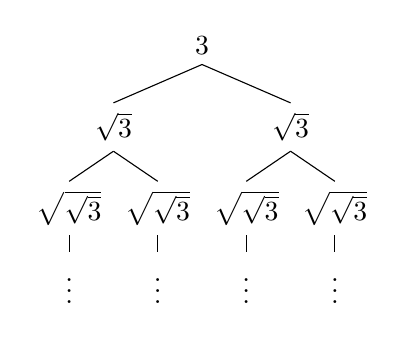
\begin{tikzpicture}
	\Tree
	[.$3$
		[.$\sqrt{3}$
			[.$\sqrt{\sqrt{3}}$ \vdots\\
			]
			[.$\sqrt{\sqrt{3}}$ \vdots\\
			]
		]
		[.$\sqrt{3}$
			[.$\sqrt{\sqrt{3}}$ \vdots\\
			]
			[.$\sqrt{\sqrt{3}}$ \vdots\\
			]
		]
	]
\end{tikzpicture} \\
There are $\log{\log{n}}$ layers in this tree. \\
By analyzing this tree, I noticed that the $k^{th}$ layer sums to $2^k * 3^{\frac{1} {2^k}}$ and each layer has a greater sum than the one above it. This means that the last layer dominates the layers above it and we can analyze this relation by finding the sum of the last row. To get the sum of the last row, I assigned $k = \log{\log{n}}$ and so the layer sums to $2^{\log{\log{n}}} * 3^{\frac{1} {2^{\log{\log{n}}}}} = \log{n} * 3^{\frac{1} {\log{n}}} \in \Theta(\log{n})$. \\
\end{proof}
\end{enumerate}



\newpage
\section*{4. Recurrence Relations Part II}
\begin{enumerate}[label=(\alph*)]
\item
\begin{enumerate}[label=(\roman*)]
\item
$\Theta(n^2)$.
\begin{proof}
Using the master theorem on $T(n) = 3T(\frac{n} {4}) + 4n^2$, we get that $d = 2$ and $\log_b{a} = \log_4{3} \approx 0.7925$. Since $d > \log_b{a}$, we get the case of the master theorem which states that if $d > \log_b{a}$, then the $\Theta$ bound for $T(n)$ is $\Theta(n^d) = \Theta(n^2)$.
\end{proof}

\item
$\Theta(n^{\log_3{45}})$.
\begin{proof}
Using the master theorem on $T(n) = 45T(\frac{n} {3}) + 0.1n^3$, we get that $d = 3$ and $\log_b{a} = \log_3{45} \approx 3.4650$. Since $d < \log_b{a}$, we get the case of the master theorem which states that if $d < \log_b{a}$, then the $\Theta$ bound for $T(n)$ is $\Theta(n^{\log_b{a}}) = \Theta(n^{\log_3{45}})$.
\end{proof}

\item
$\Theta(\log{n})$
\begin{proof}
The recurrence relation of $T(n) = 2T(\sqrt{n}) + 5$, and $T(2) = 5$ can be expressed by the following tree where each layer represents an expansion. \\
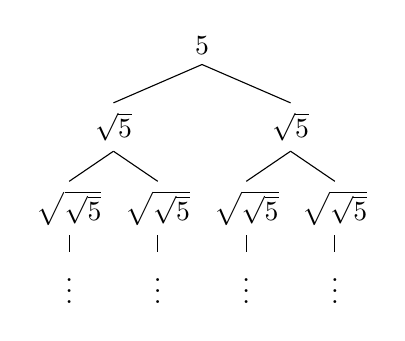
\begin{tikzpicture}
	\Tree
	[.$5$
		[.$\sqrt{5}$
			[.$\sqrt{\sqrt{5}}$ \vdots\\
			]
			[.$\sqrt{\sqrt{5}}$ \vdots\\
			]
		]
		[.$\sqrt{5}$
			[.$\sqrt{\sqrt{5}}$ \vdots\\
			]
			[.$\sqrt{\sqrt{5}}$ \vdots\\
			]
		]
	]
\end{tikzpicture} \\
There are $\log{\log{n}}$ layers in this tree. \\
By analyzing this tree, I noticed that the $k^{th}$ layer sums to $2^k * 5^{\frac{1} {2^k}}$ and each layer has a greater sum than the one above it. This means that the last layer dominates the layers above it and we can analyze this relation by finding the sum of the last row. To get the sum of the last row, I assigned $k = \log{\log{n}}$ and so the layer sums to $2^{\log{\log{n}}} * 5^{\frac{1} {2^{\log{\log{n}}}}} = \log{n} * 5^{\frac{1} {\log{n}}} \in \Theta(\log{n})$. \\
\end{proof}
\end{enumerate}
\item
\begin{enumerate}[label=(\roman*)]
\item
$\Theta(n^2\log{n})$
\begin{proof}
The recurrence relation of $T(n) = 2T(\frac{n} {2}) + n\log{n}$ can be expressed by the following tree where each layer represents an expansion. \\
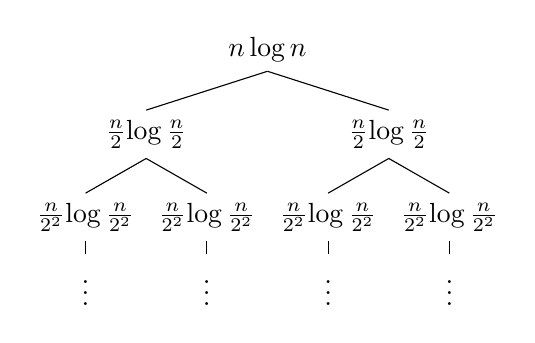
\begin{tikzpicture}
	\Tree
	[.$n\log{n}$
		[.${\frac{n} {2}}{\log{\frac{n} {2}}}$
			[.${\frac{n} {2^2}}{\log{\frac{n} {2^2}}}$ \vdots\\
			]
			[.${\frac{n} {2^2}}{\log{\frac{n} {2^2}}}$ \vdots\\
			]
		]
		[.${\frac{n} {2}}{\log{\frac{n} {2}}}$
			[.${\frac{n} {2^2}}{\log{\frac{n} {2^2}}}$ \vdots\\
			]
			[.${\frac{n} {2^2}}{\log{\frac{n} {2^2}}}$ \vdots\\
			]
		]
	]
\end{tikzpicture} \\
I have also noticed that $\frac{n} {2}{\log{\frac{n} {2}}} = \frac{n} {2}{(\log{n} - \log{2})} = \frac{n} {2}{(\log{n} - 1)}$ and $\frac{n} {2^2}{\log{\frac{n} {2^2}}} = \frac{n} {2^2}{(\log{n} - \log{2^2})} = \frac{n} {2}{(\log{n} - 2)}$ and so $\frac{n} {2^i}{\log{\frac{n} {2^i}}} = \frac{n} {2^i}{(\log{n} - \log{2^i})} = \frac{n} {2}{(\log{n} - i)}$. \\
There are $\log{n}$ layers in this tree. \\
By analyzing this tree, I noticed that the top layer has a greater sum than the layers below it so we can analyze this relation by finding the sum of all rows. I have also noticed that the sum of the top three rows is $(n\log{n}) + (n\log{n - 1}) + (n\log{n - 2}) = (n\log{n} - 0n) + (n\log{n} - 1n) + (n\log{n} - 2n)$. This leads us to the sum of all rows from the top row to the bottom: \\
\begin{align*}
(n\log{n} - 0n) + (n\log{n} - 1n) + (n\log{n} - 2n) + ... + (n\log{n} - k)
\end{align*}
\begin{align*}
= ((\log{n}) * n\log{n}) + {(-n){\sum\limits_{i = 0}^{\log{n}} i}}
\end{align*}
\begin{align*}
= n(\log{n})^2 + (-n)(\frac{n} {2} (\log{n} + 1))
\end{align*}
\begin{align*}
= n(\log{n})^2 - \frac{n^2} {2}(\log{n} + 1) \in \Theta(n^2\log{n})
\end{align*}
\end{proof}

\item
$T(n) = \Theta(n^2(\log{n})^{4})$
\begin{proof}
Using the general master theorem on $T(n) = 9T(\frac{n} {3}) + n^2(\log{n})^3$, I noticed that $T(n)$ can be formatted like $T(n) = aT(\frac{n} {b}) + f(n)$ where $a \geq 1$, $b > 1$, and $f(n) = \Theta(n^c(\log{n})^{k})$ where $c = \log_b{a}$, which means that $T(n) = \Theta(n^c(\log{n})^{k + 1})$. \\
\begin{align*}
T(n) = 9T(\frac{n} {3}) + n^2(\log{n})^3
\end{align*}
This can be rewritten as: \\
\begin{align*}
T(n) = aT(\frac{n} {b}) + f(n) 
\end{align*}
where $a = 9$, $b = 3$, $f(n) = n^2(\log{n})^3$ where $c = \log_b{a} = \log_3{9} = 2$, and $k = 3$.\\
Therefore, the general Master theorem gives: \\
\begin{align*}
T(n) = \Theta(n^c(\log{n})^{k + 1}) = \Theta(n^2(\log{n})^{3 + 1}) = \Theta(n^2(\log{n})^{4})
\end{align*}
\end{proof}
\end{enumerate}
\end{enumerate}



\newpage
\section*{5. Two Sorted Arrays}
\begin{FourPartSolution}
\begin{mainIdea}
To find the $k^{th}$ smallest element in two sorted arrays of the same length, you find points in both sorted lists that you can compare values to. The first points will just be the values in the middle of the two lists. When recursing, we will also eliminate parts of either arrays because we know that some parts of the arrays won't need to be looked at. This will also affect the $k^{th}$ value we look for so we need to change our $k$ based on whether or not the points overshot or undershot k.
\end{mainIdea}
\begin{pseudocode}
\begin{lstlisting}
\\ finding the kth smallest in array1 and array2
\\ where both are sorted lsits
kth_smallest(array1[], array2[], int k):
	\\ base case: if there is no more for array1
	\\ then just return the array2[k] because array2 is sorted already
	if length(array1) == 0:
		return array2[k]
	\\ base case: if there is no more for array2
	\\ then just return the array1[k] because array1 is sorted already
	else if length(array2) == 0:
		return array1[k]

	\\ split1 and split2 are for splitting the arrays
	\\ when I have eliminated some parts of the arrays for 
	\\recursion (split1 and split 2 start at the middle of the arrays)
	\\ also length(array1) == length(array2)
	split1, split2 = length(array1) / 2

	\\ we are finding kth smallest so when split1 + split2 < k
	\\ that means we have yet to reach k (undershot k)
	if split1 + split2 < k:
		\\ comparing numbers in the respective arrays
		\\ at their positions
		\\ when # in array1 > # in array2
		\\ then we know that we don't need to look 
		\\ at the values below array2[split2]
		\\ since we undershot k
		\\ our k also changes because
		\\ we are looking for a new kth smallest
		if array1[split1] > array2[split2]:
			array2 = array2[split2 + 1] -> array2[length - 1]
			k = k - split2 - 1
			return kth_smallest(array1, array2, k)
		\\ when # in array1 <= # in array2
		\\ then we know that we don't need to look 
		\\ at the values below array1[split1]
		\\ since we undershot k
		\\ our k also changes because
		\\ we are looking for a new kth smallest
		else:
			array1 = array1[split1 + 1] -> array1[length - 1]
			k = k - split1 - 1
			return kth_smallest(array1, array2, k)
	\\ we are finding kth smallest so when split1 + split2 >= k
	\\ that means we have overshot our split1 and split2
	\\ and so we will reduce our sizes when we recurse
	else:
		\\ comparing numbers in the respective arrays
		\\ at their positions
		\\ when # in array1 > # in array2 then we know
		\\ that we don't need to look at the values
		\\ above array1[split1] since we overshot k
		if array1[split1] > array2[split2]:
			array1 = array2[0] -> array1[split1]
			return kth_smallest(array1, array2, k)
		\\ when # in array1 <= # in array2 then we know
		\\ that we don't need to look at the values
		\\ above array2[split2] since we overshot k
		else:
			array2 = array2[0] -> array2[split2]
			return kth_smallest(array1, array2, k)
\end{lstlisting}
\end{pseudocode}
\begin{proofOfCorrectness}
The idea is correct because each time we recurse through the function, we can get rid of parts of one array. This means that there are $\Theta(\log{(length(array1))})$ for array1 and $\Theta(\log{(length(array2))})$ for array2. Since the trimmings of the arrays can alternate, then we get $\Theta(\log{(length(array1) * length(array2))}$.
\end{proofOfCorrectness}
\begin{runTime}
$\Theta(\log{(length(array1) * length(array2))}$.
\end{runTime}
\begin{justification}
When we recurse, we will trim the size of one array at a time (but for both arrays) by half so that is why there is $\log{(length(array1) * length(array2))}$.
\end{justification}
\end{FourPartSolution}



\newpage
\section*{6. Merged Median}
\begin{FourPartSolution}
\begin{mainIdea}
Just like in number 5, use divide and conquer to solve for the medians.
\end{mainIdea}
\begin{pseudocode}
\begin{lstlisting}
\\ for solving when given just 2 arrays
getMedian(array1[], array2[], int n):
	\\ get the median of the first array
    m1 = median(array1, n)
    \\ get the median of the second array
    m2 = median(array2, n)
    \\ if m1 < m2 then median must exist in half part of array1
    \\ and half part of array2[....m2]
    if m1 < m2:
        if n % 2 == 0:
            return getMedian(array1 + (n / 2) - 1, array2, n - (n / 2) +1)
        return getMedian(array1 + (n / 2), array2, n - (n / 2))
    \\ if m1 > m2 then median must exist in half part of array1
    \\ and half part of array2
    if n % 2 == 0:
        return getMedian(array2 + (n / 2) - 1, array1, n - (n / 2) + 1)
    return getMedian(array2 + (n / 2), array1, n - (n / 2))

\\ to solve for when given k arrays then you need to run the function k times.
\\ pseudocode idea based off of wiki (https://en.wikipedia.org/wiki/Median_of_medians)
\end{lstlisting}
\end{pseudocode}
\begin{proofOfCorrectness}
It is correct because the divide and conquer approach with just 2 arrays is just like the same proof as in question number 5. However, the pseudocode does not account for $k$ arrays but to account for it you need to run the pseudocode $\Theta(k)$ times.
\end{proofOfCorrectness}
\begin{runTime}
$\Theta(k\log{n})$.
\end{runTime}
\begin{justification}
The pseudocode runs it with just 2 arrays with a divide and conquer approach so it gets to be $\Theta(\log{n})$ To get it to run it with k arrays, then you need to run it $\Theta(k)$ times which makes the final answer $\Theta(k\log{n})$.
\end{justification}
\end{FourPartSolution}



\end{document}
